\vspace{-3mm}
\begin{figure}
\only<1-6>{
\begin{tikzpicture}
\begin{axis}[width=7cm,
            height=4.5cm,
            axis y line=center,
            axis x line=middle,
            xmax=4, 
            ymin=0,
            ymax=53,
            xlabel=iteration ($k$), 
            ylabel=virtual precision ($p_k$), 
            ylabel near ticks, 
            xlabel near ticks,
            xticklabels={0,0,,,,$n$},
] 

\only<1>{
\addplot[mark=none, green, ultra thick, opacity=.3] coordinates {(0,26) (4,26)};
\node[draw, green, opacity=.3] at (axis cs:2,34) {(8,26)};
\node[draw, red] at (axis cs:3,10) {X};
}
\only<2>{
\addplot[mark=none, green, ultra thick, opacity=.3] coordinates {(0,40) (4,40)};
\node[draw, green, opacity=.3] at (axis cs:2,32) {(8,40)};
\node[draw, red] at (axis cs:3,10) {X};
}
\only<3>{
\addplot[mark=none, green, ultra thick, opacity=.3] coordinates {(0,47) (4,47)};
\node[draw, green, opacity=.3] at (axis cs:2,39) {(8,47)};
\node[draw, black!30!green] at (axis cs:3,10) {V};
}
\only<4>{
\addplot[mark=none, green, ultra thick, opacity=.3] coordinates {(0,44) (4,44)};
\node[draw, green, opacity=.3] at (axis cs:2,36) {(8,44)};
\node[draw, red] at (axis cs:3,10) {X};
}
\only<5>{
\addplot[mark=none, green, ultra thick, opacity=.3] coordinates {(0,45) (4,45)};
\node[draw, green, opacity=.3] at (axis cs:2,37) {(8,45)};
\node[draw, red] at (axis cs:3,10) {X};
}
\only<6>{
\addplot[mark=none, green, ultra thick, opacity=.3] coordinates {(0,47) (4,47)};
\node[draw, green, opacity=.3] at (axis cs:2,39) {(8,47)};
\node[draw, black!30!green] at (axis cs:3,10) {V};
}
\end{axis}
\end{tikzpicture}
}


\only<7-13>{

\begin{tikzpicture}
\begin{axis}[width=7cm,
            height=4.5cm,
            axis y line=center,
            axis x line=middle,
            xmax=4, 
            ymin=-1,
            ymax=53,
            xlabel=iteration ($k$), 
            ylabel=virtual precision ($p_k$), 
            ylabel near ticks, 
            xlabel near ticks,
            xticklabels={0,,,$\frac{n}{2}$,,$n$},
] 

\only<7>{
\addplot[mark=none, blue, ultra thick, opacity=.3] coordinates {(0,47) (2,47)};
\addplot[mark=none, blue, ultra thick, opacity=.3] coordinates {(2,47) (4,47)};
\node[draw, blue, opacity=.3] at (axis cs:1,39) {(8,47)};
\node[draw, blue, opacity=.3] at (axis cs:3,39) {(8,47)};
\node[draw, black!30!green] at (axis cs:3,10) {V};
};

\only<8>{
\addplot[mark=none, blue, ultra thick, opacity=.3] coordinates {(0,23) (2,23)};
\addplot[mark=none, blue, ultra thick, opacity=.3] coordinates {(2,47) (4,47)};
\node[draw, blue, opacity=.3] at (axis cs:1,31) {(8,23)};
\node[draw, blue, opacity=.3] at (axis cs:3,39) {(8,47)};
\node[draw, black!30!green] at (axis cs:3,10) {V};
};

\only<9>{
\addplot[mark=none, blue, ultra thick, opacity=.3] coordinates {(0,11) (2,11)};
\addplot[mark=none, blue, ultra thick, opacity=.3] coordinates {(2,47) (4,47)};
\node[draw, blue, opacity=.3] at (axis cs:1,19) {(8,11)};
\node[draw, blue, opacity=.3] at (axis cs:3,39) {(8,47)};
\node[draw, black!30!green] at (axis cs:3,10) {V};
}

\only<10>{
\addplot[mark=none, blue, ultra thick, opacity=.3] coordinates {(0,4) (2,4)};
\addplot[mark=none, blue, ultra thick, opacity=.3] coordinates {(2,47) (4,47)};
\node[draw, blue, opacity=.3] at (axis cs:1,12) {(8,4)};
\node[draw, blue, opacity=.3] at (axis cs:3,39) {(8,47)};
\node[draw, black!30!green] at (axis cs:3,10) {V};
}

\only<11>{
\addplot[mark=none, blue, ultra thick, opacity=.3] coordinates {(0,4) (2,4)};
\addplot[mark=none, blue, ultra thick, opacity=.3] coordinates {(2,23) (4,23)};
\node[draw, blue, opacity=.3] at (axis cs:1,12) {(8,4)};
\node[draw, blue, opacity=.3] at (axis cs:3,31) {(8,23)};
\node[draw, red] at (axis cs:3,10) {X};
}

\only<12>{
\addplot[mark=none, blue, ultra thick, opacity=.3] coordinates {(0,4) (2,4)};
\addplot[mark=none, blue, ultra thick, opacity=.3] coordinates {(2,35) (4,35)};
\node[draw, blue, opacity=.3] at (axis cs:1,12) {(8,4)};
\node[draw, blue, opacity=.3] at (axis cs:3,27) {(8,35)};
\node[draw, red] at (axis cs:3,10) {X};
}

\only<13>{
\addplot[mark=none, blue, ultra thick, opacity=.3] coordinates {(0,4) (2,4)};
\addplot[mark=none, blue, ultra thick, opacity=.3] coordinates {(2,47) (4,47)};
\node[draw, blue, opacity=.3] at (axis cs:1,12) {(8,4)};
\node[draw, blue, opacity=.3] at (axis cs:3,39) {(8,47)};
\node[draw, black!30!green] at (axis cs:3,10) {V};
}
\end{axis}
\end{tikzpicture}

}

\only<14>{

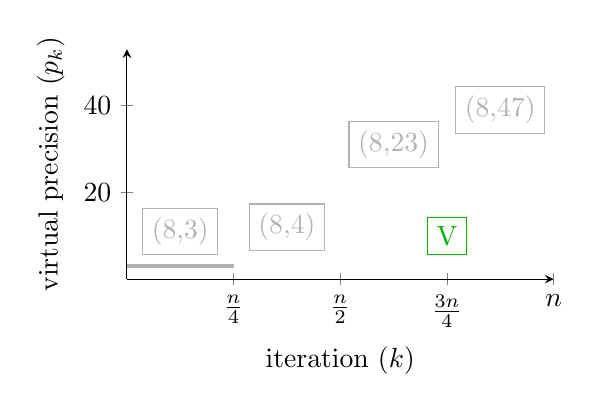
\begin{tikzpicture}
\begin{axis}[width=7cm,
            height=4.5cm,
            axis y line=center,
            axis x line=middle,
            xmax=4, 
            ymin=0,
            ymax=53,
            xlabel=iteration ($k$), 
            ylabel=virtual precision ($p_k$), 
            ylabel near ticks, 
            xlabel near ticks,
            xticklabels={0,0,$\frac{n}{4}$,$\frac{n}{2}$,$\frac{3n}{4}$,$n$},
]
\only<14>{
\addplot[mark=none, black, ultra thick, opacity=.3] coordinates {(0,3) (1,3)};
\node[draw, opacity=.3] at (axis cs:.5,11) {(8,3)};
\addplot[mark=none, black, ultra thick, opacity=.] coordinates {(1,4) (2,4)};
\node[draw, opacity=.3] at (axis cs:1.5,12) {(8,4)};
\addplot[mark=none, black, ultra thick, opacity=.] coordinates {(2,23) (3,23)};
\node[draw, opacity=.3] at (axis cs:2.5,31) {(8,23)};
\addplot[mark=none, black, ultra thick, opacity=.] coordinates {(3,47) (4,47)};
\node[draw, opacity=.3] at (axis cs:3.5,39) {(8,47)};
\node[draw, black!30!green] at (axis cs:3,10) {V};
}

\end{axis}
\end{tikzpicture}

}


\only<15>{

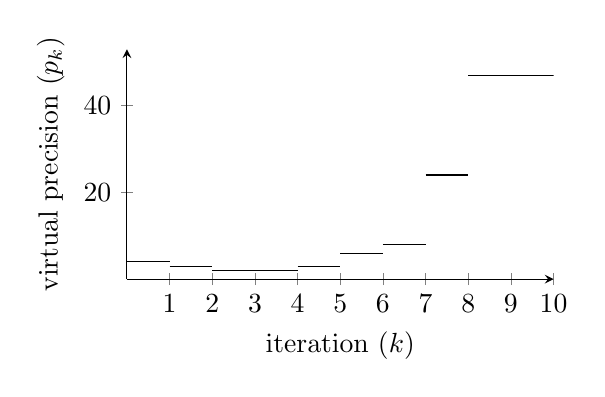
\begin{tikzpicture}
\begin{axis}[width=7cm,
            height=4.5cm,
            axis y line=center,
            axis x line=middle,
            xmax=10, 
            ymin=0,
            ymax=53,
            xlabel=iteration ($k$), 
            ylabel=virtual precision ($p_k$), 
            ylabel near ticks, 
            xlabel near ticks,
            xtick={0,1,2,3,4,5,6,7,8,9,10},
            xticklabels={0,1,2,3,4,5,6,7,8,9,10},
]
\only<15>{
\addplot[mark=none, black] coordinates {(0,4) (1,4)};
\addplot[mark=none, black] coordinates {(1,3) (2,3)};
\addplot[mark=none, black] coordinates {(2,2) (3,2)};
\addplot[mark=none, black] coordinates {(3,2) (4,2)};
\addplot[mark=none, black] coordinates {(4,3) (5,3)};
\addplot[mark=none, black] coordinates {(5,6) (6,6)};
\addplot[mark=none, black] coordinates {(6,8) (7,8)};
\addplot[mark=none, black] coordinates {(7,24) (8,24)};
\addplot[mark=none, black] coordinates {(8,47) (9,47)};
\addplot[mark=none, black] coordinates {(9,47) (10,47)};
}

\end{axis}
\end{tikzpicture}

}

\end{figure}
